\section{Study Setting}\label{sec:Methodology}

%\todo[inline]{O objetivo não é esse. O nosso objetivo é compreender
%  como uma abordagem, que explora dados de tráfego de rede, pode melhorar
%  a acurácia do \mas na detecção de malware.}

In this section, we present \droidxpflow, a framework for Android malware detection by analyzing the network flow. Our goal with \droidxpflow is to build an in-depth understanding of the network traffic generated by benign and malicious apps, and understand how an approach based on network flow analysis and ML can improve the accuracy of malware classification. To achieve this goal, we investigate the following research questions:

%\todo[inline]{As questões de pesquisa não estão bem formuladas. Primeiro,
%  questões do tipo 'yes' ou 'no' não nos apoia em um trabalho acadêmico,
%  melhor 'To what extent \ldots'. As outras questões estão genéricas.
%  Temos que estabelecer uma relação com mining sandbox}

\begin{enumerate}[(RQ1)]
\item \rqa
\item \rqb
\item \rqc
% \review{\item \rqe}
\end{enumerate}

To this end, we present how \droidxpflow collects data from network traffic, while executing test case generation tools (Section~\ref{sec:data}). In Section~\ref{sec:feature} and Section~\ref{sec:set} we explain how we extract and preprocess the features from our dataset. Finally, we describe the procedures we used to classify repackage apps as malware or non-malware, based on network traffic data and ML approach (Section~\ref{sec:learning}).

\subsection{Preliminaries}\label{sec:dataset}

%\todo[inline]{Precisamos discutir aqui como nós construímos o dataset? Isso não faz parte do artigo anterior?.
%  Podemos publicar esse dataset no Zenodo, ou no IEEE Data (https://ieee-dataport.org/submit-dataset). Podemos revisar
%um pouco aqui \ldots. Um cuidado, repack é um subset de AndroZoo.}

%\todo[inline]{Confuso. Temos 4,076 apps, sendo 1,777 originl and 4,076 repackaged. Frases como essa
%  exigem demais do leitor.}

To test and evaluate our proposal, we used the same dataset (\cds) described in Chapter 5. As mentioned in the previous chapter, it contains 5,844 real-world apps from two repositories of repackaged Android apps:(\repack~\cite{DBLP:journals/tse/LiBK21} and \amc~\cite{rafiq2022andromalpack}). Of these, 1,777 are original versions and 4,067 are repackaged versions, with multiple repackaged versions of the same original app possibly coexisting within the \cds dataset. According to VirusTotal, at least two security engines identified 2,886 out of the 4,067 repackaged apps as malware ($70.96$\%), while 1,181 are benign. The \cds dataset contains several features related to the apps, including information about malware families and the similarity between the original and repackaged versions of each app. Further details about the \cds dataset and how they were obtained can be found in Chapter 5 of this thesis.

This study aims to identify malicious behavior in repackaged Android apps within the \cds dataset, using \droidxpflow and analyzing network traffic features with ML techniques. The overview architecture of the proposed method is presented in Figure~\ref{fig:arq}. The entire process involves three main phases: data collection (normal and malware traffic), feature extraction and selection, and model training and classification. During the data collection phase, we capture all the traffic from both the original and repackaged apps and store the generated PCAP files in a traffic store. In the next step, we extract features from the PCAP files in the repository and select the most relevant ones for the model. Finally, the prepared dataset is fed into the ML algorithm to train and classify the samples as either malicious or benign. The following sections, provide more details of proposed work.


\subsection{Data Collection}\label{sec:data}

The DroidXP~\cite{DBLP:conf/scam/CostaMCMVBC20} tool was initially designed to compare test case generation tools in terms of identifying malicious app behaviors using the \mas. This makes it a relevant tool for automating data collection for both static and dynamic analysis, following the steps outlined below:


%\todo[inline]{Não sei. acho que essa parte deveria estar em background. talvez de forma mais resumida.}

%\todo[inline]{Outra op\c c\~{a}o \'{e} termos uma se\c c\~{a}o sobre Data Collection, e iniciarmos essa
%  indicando que usamos duas estrat\'{e}gias de coleta de dados. Uma que coleta as informa\c c\~{o}es de
%  APIa sens\'{i}veis e outra que coleta o tr\'{a}fego de rede. Quebrar\'{i}amos as disucss\~{o}es
%espec\'{i}ficas em subsubse\c c\~{o}es. }

%\todo{inline}{Essa terminologia 'demonstrade' eh muito forte. Em vez de 'As demonstrade in the study (nao sei qual o estudo)', DroidXP can compare', poderia ser 'DroidXP was initially designe to compare \ldots'.}


%\todo{inlilne}{Vamos ser mais diretos. Em vez de 'the \fhc uses', coloca logo 'DroidXP instruments'. Acho que devemos remover alguns detalhes desse paper, e citar os outros trabalhos. Exemplo de talhes, 'As noted by the authors'. Outra coisa, estamos exigindo muito do leitor saber quem sao os autores, qual estudo estamos nos referindo, \ldots}

\begin{enumerate}[1.]
 \item \textbf{Instrumentation}:  All apps analyzed are instrumented to collect relevant information before execution. In the background, DroidXP leverages DroidFax~\cite{DBLP:conf/icsm/CaiR17a} to gather static information about the apps being analyzed.
 
   %\todo[inline]{Confuso essa parte inicial do texto ``As statistical result show that \ldots''. Na verdade, o par\'{a}grafo inteiro est\'{a} super confuso. Eu diria que toda essa se\c c\~{a}o MAS Data Collection deveria ser re-escrita. Quem \'{e} 'the author'?}
   
 \item \textbf{Execution}: DroidXP installs the instrumented versions of the apps on an Android emulator and restarts it before the actual execution. It then initiates a test case generation tool to execute all the apps and collect the dynamic data from the pre-programmed executions setup.
  
%\todo[inline]{A se\c c\~{a}o \'{e} sobre data collection. Vamos simplificar essa se\c c\~{a}o, deixa-la mais atrativa para um leitor.}   

\item \textbf{Data Collection}: At the end of the execution step, DroidXP again utilizes DroidFax, this time to compile all relevant information from the execution step, such as calls to sensitive APIs, and more. This step, and previous are crucial for dynamic analysis.
\end{enumerate}

For our study, we extended the original version of DroidXP by adding new functionality to its execution phase. This extension (\droidxpflow) now uses the TcpDump tool to collect both inbound and outbound network traffic. Now its possible, with \droidxpflow support, capture data for network traffic in (PCAP)~\cite{DBLP:conf/iv/UhlarHR21} format, for all the apps analyzed.


As described in Section~\ref{sec:introduction}, previous studies have shown that $86\%$ of Android malware is found in repackaged original appss~\cite{DBLP:journals/tdsc/TianYRTP20,DBLP:conf/sp/ZhouJ12}. For this reason, we decided to collect the network traffic data generated exclusively by repackaged samples from the \cds dataset, which contains $4,067$ samples ($2,886$ malicious and $1,181$ benign), as detailed in Section~\ref{sec:dataset}. To capture the network traffic data, we followed the same criteria explained in the previous chapter, that is: each selected app was executed using \droidxpflow, using the test case generation tool DroidBot~\cite{DBLP:conf/icse/LiYGC17}, over a period of $3$ minutes for each app.

At the end of the data collection phase, we have multiple PCAP files, each corresponding to an analyzed app. A PCAP file contains copies of network packets, enabling dynamic analysis of both payloads and packet headers~\cite{DBLP:conf/iv/UhlarHR21}. Since storing and processing PCAP files is resource-intensive, it is necessary to perform a limited analysis of network segments rather than analyzing all of them. To extract the most relevant features for our study, as a first step we use CICflowMeter~\cite{DBLP:conf/icissp/LashkariDMG17} software, as described in the next section.


%Figure~\ref{fig:mine} show a overview of \mas data collection.


%\todo[inline]{Por que sandbox? Estamos sendo corretos aqui?}
%The study consider that a sandbox of app identifies a malware whenever the malicious app version makes a call to a sensitive API, which was not called during the exploratory phase of your original version, as present at Figure~\ref{fig:mine}.


\begin{figure*}[h]
  \centering
  
    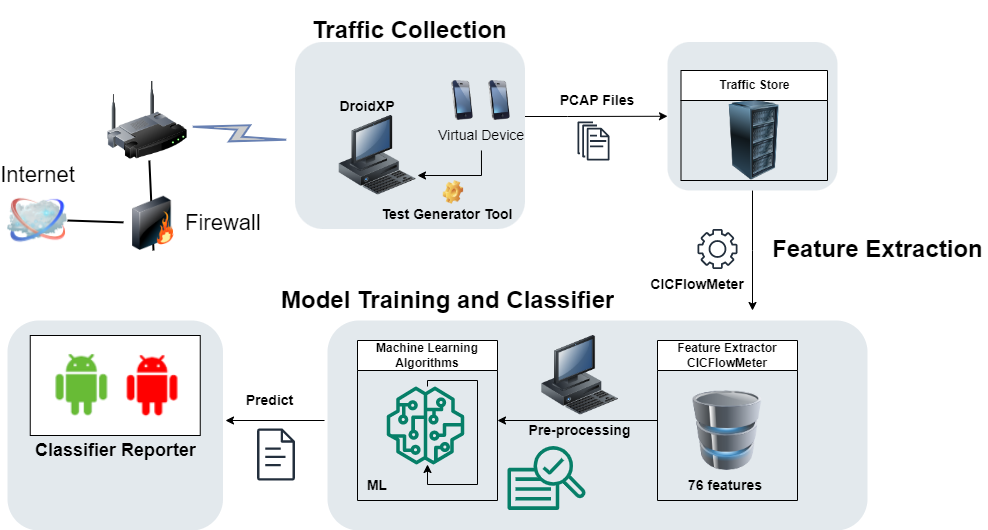
\includegraphics[width=0.80\textwidth]{image/archic.png} \\[\abovecaptionskip]
    
  \caption{Overview architecture of the \droidxpflow Framework proposed for malware detection}\label{fig:arq}
\end{figure*}




%\todo[inline]{Aqui temos que dizer como eh a arquitetura dessa solu\c c\~{a}o. DroidXP foi usado 'as is', ou foi adaptado? Caso a gente esteja usando o DroidXP para coletar as duas coisas (apis sensiveis e trafego), devemos iniciar a se\c c\~{a}o indicando que adaptamos a vers\~{a}o do DroidXP de~\cite{}. A vers\~{a}o anterior coletava apenas as APIs sens\'{i}veis (descreve como era feito, de forma resumida). Com a adapta\c c\~{a}o, foi poss\'{i}vel coletar tamb\'{e}m informa\c c\~{o}es de tr\'{a}fego de redes. Nesse ponto voce comeca a discutir a parte de coleta de trafego de redes.}



%\todo[inline]{Por que n\~{a}o deixamos 'feature-extraction' como data collection?}
%\subsubsection{Feature Extraction}\label{sec:extraction}

%\todo[inline]{A pior coisa do mundo eh indicar que gera 86 feature e nao vai descreve-las por falta de espa\c co. Aqui pode ser escrito algo como '86 features, incluindo A, B, C.' Dessas 86 foram excluidas ABC features, por cause de \ldots. Outras XYZ foram excluidas pode \ldots. In the end, we considered only \ldots.}
\subsection{Feature Extraction}\label{sec:feature}

To extract features, we processed each traffic file (PCAP file) generated by \droidxpflow during the data collection step using the CICFlowMeter tool. This tool extracts feature sets in CSV format from the corresponding PCAP file. In the end, we combined all the CSV files into a single file containing a total of 86 features, including flow duration, destination port, number of transmitted bytes, and more. We did not consider all of these features, removing those that were irrelevant to our study, such as Flow ID, Source IP, Destination IP, Source Port, Source MAC, Destination MAC, Protocol, and Timestamp. In the end, we considered 78 features.

%\todo[inline]{Trabalho de doutorado. Precisamos justificar essas decis\~{o}es. Temos que explicar o que eh destination port, porque ela eh relevante, \ldots. Preferencialmente suportar essa decis\~{a}o por trabalhos anteriores.}

In a second step, we filtered our initial CSV file based on ``Destination Port''. Destination port numbers categorize the service being used in the traffic and is an important feature for analyzing network flow and potential malicious behavior~\cite{DBLP:journals/compsec/UmerSB17,DBLP:journals/comsur/SperottoSSMPS10}. Malware can often exploits ports such as 443 (HTTPS), 53 (DNS), or 80 (HTTP) to communicate with Command \& Control (C\&C) servers, carry out exploits, or blend in with normal traffic~\cite{DBLP:journals/comsur/SperottoSSMPS10}. Various datasets used to evaluate flow-based approaches include this important feature, like: CIDDS-001~\cite{Ring2017FlowbasedBD}, CICIDS17~\cite{DBLP:conf/icict/MahfouzVS19} and CTU-13~\cite{DBLP:journals/compsec/GarciaGSZ14}. Considering the importance of this feature, we explored the six most relevant destination ports, which appear most frequently in our initial CSV file, accounting for $74.25\%$ of all network traffic captured. (see Table~\ref{tab:port}).

\begin{table}[h]
  \caption{THE 6 MOST RELEVANT DESTINATION PORT.}
  \centering
  \begin{small}
    \begin{tabular}{rrlr}   \hline
 \# & Port & Description & Occurs  \\ \hline

1 &  443 &  Hypertext Transf. Protocol Secure &  1275293  \\ 
  2 &  53 & Domain Name System & 641965  \\ 
  3 &  80 & Hypertext Transfer Protocol &  38830  \\ 
  4 &  853 & DNS over TLS &  32784  \\ 
  5 &  5228 & Google Cloud Messaging &  26509  \\ 
  6 &  123 & Network Time Protocol & 9179  \\ 
  
   \hline

 \end{tabular}
 \end{small}
 \label{tab:port}
 \end{table}


\begin{table}[ht]
  \caption{STATISTICAL FUNCTIONS AT FEATURES.}
  \centering
  \begin{small}
    \begin{tabular}{rllrr}   \hline
 \# & Function & Description\\ \hline

1 &  min &  Minimum\\ 
  2 &  max & Maximum\\ 
  
  3 &  mean & Average\\ 
  
  4 &  median & Median\\ 
  5 &  count & Number of observation\\ 
  6 &  var & Variance\\ 
  7 &  skew & Skewness \\ 
   \hline

 \end{tabular}
 \end{small}
 \label{tab:function}
 \end{table}

%\todo[inline]{Talvez Data Preparation, Pre-processing, \ldots. Alguma coisa que os leitores estejam mais familiarizados.}
\subsection{Data Preprocessing}\label{sec:set}

%\todo[inline]{Justificar \ldots}

According to the literature~\cite{DBLP:conf/ichmi/Xie22,DBLP:journals/mta/AmiriebrahimabadiM24}, selecting relevant features is crucial for achieving good predictive power in a ML model. This can improve model accuracy and reduce training time. However, selecting the appropriate features is not a trivial task and often requires expert knowledge. For this reason, it is more effective to allow the machine to learn which features are most important~\cite{DBLP:journals/spe/FallahB22}. In this work, we extracted a subset of statistical features (Table~\ref{tab:function}), and fed them into the model. Thereby, we group the initial 76 features (excluding Destination Port and Hash), with 6 Destination Ports, and 7 statistical features listed in Table~\ref{tab:function}. This combination greatly enhances the convenience of our experiment when we use it with ML algorithms to train detection models. By the end of this step, we have a initial dataset (here after \fds) with a total of 3,194 features ($76\times6\times7$) + Hash + Type (benign/malicious).


Still, high-dimensional datasets have a costly training time. To select the most relevant features and reduce their quantity, we took a second step by comparing the performance of four popular approaches using our initial \fds (3,194 features). We compared the performance of Linear Discriminant Analysis (LDA), Quadratic Discriminant Analysis (QDA), Logistic Regression, and the Random Forest algorithm~\cite{james2023introduction}. Subsequently, we also explored a novel classifier called the Energy-Based Flow Classifier (EFC), which is inspired by the inverse Potts model from quantum mechanics~\cite{DBLP:journals/tnsm/PontesSGBM21}.


To compare the performance of the algorithms, we train the
model based on the all 3,194 feature of \fds, and later use it for malware classification. In our learning-based classification procedure,
we split the feature set into a training set consisting of $70\%$
of the samples and a testing set consisting of $30\%$, randomly
selected from the initial \fds. The testing set is used solely
to evaluate the detection accuracy of the models. Among these methods, the supervised approach Random Forest delivered the best performance. This algorithm aggregates multiple decision trees, with each tree constructed using a random subset of features. This process decorrelates the trees, allowing for a more thorough exploration of the model and substantially improving predictive performance~\cite{james2023introduction}.

To achieve the best-fitting model, we also varied several model parameters using cross-validation~\cite{DBLP:phd/us/Stephenson22} on the training data. Cross-validation is a technique commonly used in ML to assess how well a model performs on an independent dataset~\cite{DBLP:journals/jsan/AwadF23}. This technique tests the model on different subsets of the data, helping to detect overfitting and making efficient use of the available data. For our experiment, cross-validation proposed the following values for five parameters in the Random Forest algorithm:

\begin{itemize}
    \item Number of trees in the forest: $190$
    \item The minimum number of samples required to split an internal node: $18$
    \item The minimum number of samples required to be at a leaf node: $3$
    \item The number of features to consider when looking for the best split: $\log_2(features)$
    \item The maximum depth of the tree: None~\footnote{If None, then nodes are expanded until all leaves}
\end{itemize}

Finally, using the Random Forest model with the parameters suggested by the cross-validation technique, we selected the 20 most relevant features based on Gini Importance, or Mean Decrease in Impurity (MDI)~\cite{james2023introduction}. With this procedure, we reduce training time by disregarding features that contribute little to the model, while at the same time improve the model accuracy in $7\%$. In the end, our final \fds have the follow selected features listed in Table~\ref{tab:features}.


%\todo[inline]{N\~{a}o poderia ser usado para justificar as decis\~{o}es da se\c c\~{a}o anterior? Aqui ja fala em Random Forest, mas eh algo que vai ser discutido mais na frente. }


\begin{table*}[ht]
  \caption{THE 20 MOST RELEVANT FEATURES.}
  \centering
  \begin{small}
    \begin{tabular}{rrlrrr}   \hline
 \# & Feature & Description & Function & Port &  Weights  \\ \hline

	1 &  \texttt{bwd\char`_byts\char`_b\char`_avg} &Average bytes per bulk in the backward direction & median & 443& 0.391424\\ 
    2 & \texttt{flow\char`_iat\char`_min} & Minimum time between two packets sent in the flow & max  & 443 &0.033638\\ 
	3 &  \texttt{bwd\char`_byts\char`_b\char`_avg} &  Average bytes per bulk in the backward direction &  max & 5228& 0.028322\\
	4 & \texttt{fwd\char`_iat\char`_mean} & Mean time between two packets sent in the forward direction & median & 443 &0.027254\\ 
	5 & \texttt{flow\char`_byts\char`_s} & Flow rate in bytes per second & median  & 443&0.022235\\
    6 & \texttt{tot\char`_bwd\char`_pkts} & Total packets in the backward direction & mean  & 80 &0.019434\\ 
	7 &  \texttt{subflow\char`_bwd\char`_pkts} & The average number of packets in a sub flow in the bwd direr. &  mean  & 80&0.014900\\ 
	8 & \texttt{bwd\char`_header\char`_len} & Total bytes used for headers in the backward direction &  mean  & 80& 0.013488\\

	9 &  \texttt{bwd\char`_blk\char`_rate\char`_avg} & Average number of bulk rate in the backward direc. &  mean  & 443&0.009523\\
    
	10 & \texttt{flow\char`_iat\char`_std} & Standard deviation time between two packets sent in the flow &median & 443 &0.009155\\ 
 
	11 & \texttt{bwd\char`_byts\char`_b\char`_avg} & Average number of bytes bulk rate in the backward direc. & max  & 443&0.008799\\

    12 & \texttt{fwd\char`_pkts\char`_s} & Number of forward packets per second & median  & 443&0.007647\\

	13 & \texttt{bwd\char`_seg\char`_size\char`_avg} & Average size observed in the backward direction & max  & 443&0.007331\\
    	14 & \texttt{bwd\char`_pkts\char`_len\char`_mean} & Mean size of packet in backward direction & max  & 443&0.006962\\ 

15 & \texttt{flow\char`_pkts\char`_s} & Num. of bytes in the initial window in the fwd dir. &  median  & 443&0.006737\\ 

	16 & \texttt{bwd\char`_pkt\char`_len\char`_std} & Standard deviation size of packet in backward direc. & median  & 443&0.005827\\ 

	17 & \texttt{bwd\char`_pkt\char`_len\char`_std} & Standard deviation size of packet in forward direction & skew  & 443&0.005319\\
	18 & \texttt{bwd\char`_iat\char`_std} & Average size observed in the backward direction & median  & 443&0.005026\\
    	19 & \texttt{fwd\char`_iat\char`_std} & Std. deviation time between two packets sent in the forward direc. & median  & 443 &0.004147\\

    20 & \texttt{bwd\char`_blk\char`_rate\char`_avg} & Average number of bulk rate in the backward direc. & var  & 443&0.003966\\ 
	

   \hline

 \end{tabular}
 \end{small}
 \label{tab:features}
 \end{table*}


 %\todo[inline]{Essa se\c c\~{a}o poderia ser chamada de Data Analysis Procedures?}
\subsection{Model Training and Classifier}\label{sec:learning}

%\todo[inline]{N\~{a}o sei se precisamos introduzir o conceito de ML aqui. }

%\todo[inline]{Aqui deveriamos descrever apenas os m\'{e}todos usados para an\'{a}lise de dados. A menos que se queira deixar claro que Random Forest foi melhor, e os outros n\~{a}o ser\~{a}o mais discutidos no texto. Se for esse o caminho, eh necess\'{a}rio apresentar a performance dos outros aqui. Handrick, eu sugiro fortemente voce ler alguns artigos que usam ML para detectar malwere, e tentar seguir uma estrutura semelhante. Definir ML, Cross-validation, \ldots, aqui n\~{a}o eh bom. Aqui devemos deixar claro nossos metodos de analise de dados. Mas no final, sugiro ler outros artigos e tornar essa secao mais proxima dos outros artigos.}

To explain our data analysis, we divided the procedure into two steps. First, after selecting the best features for analysis, once again we split the data into a training set consisting of $70$\% of the samples, and a testing set with the remaining $30$\%, randomly selected from \fds. We then trained the selected samples using five ML algorithms explored in our study: Linear Discriminant Analysis (LDA), Quadratic Discriminant Analysis (QDA), Logistic Regression (LR), Random Forest (RF), and the Energy-based Flow Classifier algorithm (EFC). To obtain the best performance of all algorithms, we use cross-validation to obtain the best parameter set of each algorithm. After training, we provided predictions based on the model generated by each ML algorithm.

As a second step, we triangulate the results of the \ml classification, with the outputs of \vt, for each model. This may lead to one of the following situations:

\begin{itemize}
\item {\bf True Positive (TP)}. The \ml label a repackaged version as a malware and, according to
  \vt, at least two \ses label the asset as a malware. This decision aligns with existing recommendations~\cite{vt-label,DBLP:journals/ese/KhanmohammadiEH19}
   
\item {\bf False Positive (FP)}. The \ml label a repackaged version as a malware and, according to \vt, at most one \se labels the asset as a malware.

\item {\bf False Negative (FN)}. The \ml does not label a repackaged version as a malware, and according to \vt, at least two \ses label the asset as a malware.
\end{itemize}

We compute \emph{Precision}, \emph{Recall}, and \emph{F-measure} ($F_1$) from
the number of TP, FP, and FN (using standard formulae). We use basic statistics (average, median, standard deviation) to identify the accuracy of the \ml for malware classification at each model explored on the \fds dataset.
